\documentclass{report}
\usepackage[utf8]{inputenc}
\usepackage[top=1.5cm, bottom=2cm, left=3.5cm, right=3.5cm]{geometry}
\usepackage[frenchb]{babel}
\usepackage[T1]{fontenc}
\usepackage{lineno}
\usepackage{natbib}
\usepackage{float}
\usepackage{graphicx}
\usepackage{hyperref}
\usepackage{enumitem}
\usepackage{wrapfig}
\usepackage{tabularx}
\usepackage{alltt}
\usepackage{titlesec}
\usepackage{upquote}
\usepackage{listings}

\input{lang.Rnw}
\title{Rapport Projet Bigdata ISEP 2015}
\author{CHANTHAVONG Delphine \\ RASOLOMALALA Narisely \\ PHILIPPE Romain \\ DIVAD Loïc}
\date{Novembre 2015}
\usepackage{Sweave}
\begin{document}
\Sconcordance{concordance:Report.tex:Report.Rnw:%
1 22 1 1 0 82 1}


\maketitle

\tableofcontents

\listoffigures

\titleformat
{\chapter}[display] %command% shape
{\bfseries\huge} % format
{} % label
{-6ex} % sep
{
    \thechapter. 
    %\rule{\textwidth}{1pt}
    %\vspace{1ex}
    %\centering
} % before-code
[
\vspace{0ex}%
%\rule{\textwidth}{0.3pt}
] % after-code


%\newenvironment{link}[2]{\textcolor{blue}{\underline{\textit{\href{#1}{#2}}}}}{}
\newenvironment{unix}[1]{\par\begin{center}\begin{tt}\$ \emph{#1} \end{tt}\end{center}}{\par}
\newenvironment{block}[1]{\par\vspace{5pt}\underline{\emph{#1}:}} {\par\vspace{5pt}}
\newenvironment{key}[1]{\par\vspace{5pt}\underline{\emph{#1}:}} {\par\vspace{5pt}}

\edef\hc{\string:}
\newcommand{\link}[2]{\textcolor{blue}{\underline{\textit{\href{#1}{#2}}}}}
\newcommand{\sqlcmd}[1]{\begin{tt}\textcolor{NavyBlue}{#1}\end{tt}}
\newcommand{\jb}[1]{\begin{tt}\textcolor{Red}{#1}\end{tt}}

%Mulberry
\newpage


\chapter{Introduction}

\chapter{Environnement de travail, outils et organisation.}

\par
Pour pouvoir collaborer plus facilement, nous avons déployé un “cluster” Hadoop que nous installons et administrons nous-même. Cela nous a permis d’éviter des problèmes de ressources liés à l’utilisation des nombreux logiciels.
\par
Le cluster est composé de 3 serveurs \textbf{PSV1, PSV2, PSV3} (ces abréviations sont utilisées dans la suite de la description de l'environnement) sur lesquels nous avons installé la distribution Hortonworks de Hadoop (HDP 2.2) et nous permet de travailler ensemble à distance.
\par
Dans un premier temps, il nous faut connecter les serveurs entre eux. Pour cela, on génère avec le premier serveur (\textbf{PSV1}) une clé SSH qui sera copiée sur les deux autres serveurs (dans le fichier knowhost du user root).
\par
Ensuite, on débute l’installation de l’écosystème. On commence donc par l’installation d’Ambari-serveur que l’on a placée sur \textbf{PSV1}.
\par
Par la suite, lorsqu’Ambari serveur est lancé, il nous est demandé de fournir les adresses IP des deux autres serveurs du cluster. Ambari installe alors Ambari-agent sur chaque serveur qui lui se chargera d’installer tous les logiciels Hadoop (il nous propose une répartition des logiciels que l’on a ensuite adaptée à nos ressources)   

\par
\begin{block}{Note sur les agents Ambari} Il consiste en une série de scripts python dédiée à de nombreuses tâches comme l’installation des paquets, la mise en place et l'autorisation des répertoires ou encore le redémarrage des services Hadoop. 
\end{block}
Notre cluster est finalement installé. Nous présenterons donc une répartition des différents logiciels. Chaque machine possède 4GO RAM et possède un Datanode sur un file system de 1 TO. \newline

\begin{figure}[h!]
\centering
    
\begin{tabular}{|c|c|c|c|}
\hline
Note&SV1&SV2&SV3\\ \hline
&Ambari serveur&&\\ \hline
&&namenode&sec namenode\\ \hline
&&Yarn&Yarn\\ \hline
&&&Oozie\\ \hline
&&&Hbase\\ \hline
&&&Hive\\ \hline
&Zookeeper&Zookeeper&Zookeeper\\ \hline
Éteint&&Storm&\\ \hline
Éteint&&Kafka&\\ \hline
&Hue&&\\ \hline
&Livy&&\\ \hline
(client)&Tez&Tez&Tez\\ \hline
(client)&Pig&Pig&Pig\\ \hline
(client)&Sqoop&Sqoop&Sqoop\\ \hline
\end{tabular}

\caption{Répartition des logiciels}
\end{figure}





\chapter{Intégration de données}

\section{Description des fichiers}

\begin{itemize}
  \item \emph{Data integration: Explain how the data has been recovered from the EnerNOC website and  how it has been integrated into HDFS and a Hive database.}
\end{itemize}

% -- Note en pied de page
{\let\thefootnote\relax\footnotetext{
  \textsuperscript{1} Lien de téléchargement du jeu de données : 
  \begin{link}{https://open-enernoc-data.s3.amazonaws.com/anon/index.html}{Les archives}\end{link}
  }
}
%    %
{\let\thefootnote\relax\footnotetext{
  \textsuperscript{2} EnerNoc: www.enernoc.com
  }
}
%    %
{\let\thefootnote\relax\footnotetext{
  \textsuperscript{3} La correspondance entre les sites et les identifiants des fichiers est établie dans le fichier de méta data qui sera vu plus bas.
  }
}
%    %
{\let\thefootnote\relax\footnotetext{
  \textsuperscript{4} Nombre de secondes écoulées depuis 1er janvier 1970 00:00:00 UTC
  }
}
% -- Note en pied de page

\par Le dataset est hébergé sur une plateforme amazon\textsuperscript{1}. Il s'agit d'un open data, ces informations sont accessibles et utilisables par tous. Elles sont mises à disposition par EnerNoc\textsuperscript{2}, un éditeur de logiciels orienté dans la consommation d'énergie. 
\par Divers formats sont proposés par l'entreprise, mais nous avons uniquement téléchargé les sources de données au format CSV.  L'archive contenant les fichiers est alors téléchargée sur une des machines disposant d'un client Hadoop. 

\begin{unix}{wget https://open-enernoc-data.s3.amazonaws.com/anon/csv-only.tar.gz}\end{unix}

Puis décompressée:

\begin{unix}{tar -zxvf all-data.tar.gz}\end{unix}

\par On obtient alors un sous dossier de données sources et un sous dossier de "meta data"  servant à expliquer les fichiers. On rédige ici une description des fichiers.

\par Tous les fichiers portent l'extension CSV et ont pour unique titre un identifiant\textsuperscript{3}. Il y en a 100. Tous les csv ont un poids proche de 4.5 Mo ($\pm$ 0.2 Mo) pour 105409 lignes chacun. Le dossier total pèse 460 Mo. Ils présentent tous une première ligne d'en-tête et 105408 autres lignes correspondant chacune à une mesure pour un site à un instant donné. Les mesures sont prises toutes les 5min pendant un an. Ce qui signifie qu'il y a 5min entre chaque ligne du csv. Les colonnes sont les suivantes : timestamp, dttm\_utc, value, estimated, anomaly.

\begin{figure}[h!]
\centering

\begin{tabular}{|l|l|}
\hline
timestamp&Date de la mesure au format POSIX\textsuperscript{4} \\ \hline
dttm\_utc&Conversion de la date au format UTC (yyyy-MM-dd HH:mm:ss)\\ \hline
value&Consommation en kWh\\ \hline
estimated&Boolean pour savoir si la valeur est estimée\\ \hline
anomaly&Indicateur pour savoir si la valeur est erronée\\ \hline
\end{tabular}

\caption{Description des fichier xxx.csv}
\end{figure}

Ces fichiers sont à croiser avec le fichier de meta data. Il présente une ligne par site étudié. \newpage

\begin{figure}[h!]
\centering

\begin{tabular}{|l|l|}
\hline
SITE\_ID&Identifiant du site. C’est le nom du fichier contenant ces mesures.\\ \hline
INDUSTRY&Secteur du site\\ \hline
SUB\_INDUSTRY&Sous catégorie du secteur du site\\ \hline
SQ\_FT&Surface du site en pied carré\\ \hline
LAT&Latitude du site\\ \hline
LNG&Longitude du site\\ \hline
TIME\_ZONE&Nom du fuseau horaire du site\\ \hline
TZ\_OFFSET&Heure de décalage par rapport au méridien de Greenwich\\ \hline

\end{tabular}

\caption{Description du fichier all\_sites.csv}
\end{figure}

\begin{block}{Note} Dans une démarche pragmatique, avant l'insertion des données dans HDFS nous avons visualisé quelques CSV au hasard à l’aide d’outils mieux maîtrisés. Nous utilisons donc le langage python pour tirer quelques conclusions qui nous permettrons de mieux appréhender les questions. On indique dans la remarque suivante les points qui ont attiré notre attention. \end{block}

\textbf{Remarques :}
\begin{itemize}
\item[-] Il n’y a que 4 industries prises en compte
\item[-] Les industries sont bien équilibrées en nombre de sites (25sites / industrie)
\item[-] 5 fuseaux horaires différents sont répertoriés
\item[-] On trace brièvement les 2000 premiers points (7j) du site 100 (Education)
\end{itemize}

\par De toutes ces remarques découlent les intuitions suivantes. Il peut être intéressant de créer une table partitionnée par industrie. Les Load Curves peuvent varier plus ou moins entre 25 et 5 kWh en une demie journée.

\par Nous insérons maintenant le dataset dans le filesystem d’hadoop. Pour une meilleure exploitation des fichiers nous retirons les entêtes pour chaque fichier avant l’insertion. Une fois placé dans le dossier contenant les mesures, on applique la commande suivante :
\begin{unix}{ls | xargs -n 1 sed -i 1d}\end{unix}
Remarque : Même si les fichiers contenant les mesures ont un encodage correct et un délimiteur de champ/ligne
adapté, le fichier de meta données lui est problématique. En effet, les lignes sont séparées par le caractère \^{}M.
Hue propose différents délimiteurs pour les champs mais pas pour les lignes. Le problème est résolu avec la
commande suivante :
\begin{unix}{sed -i -e "s/$\backslash$r/$\backslash$n/g"}\end{unix}

Les fichiers sont alors finalement tous prêts à être insérés dans le filesystème hadoop. La partie suivante explique comment nous les avons transférés après le nettoyage. \newpage

\section{Script d’intégration}

% -- Note en pied de page
%    %
{\let\thefootnote\relax\footnotetext{
  \textsuperscript{5} Pour le projet nous nous appuyons sur la documentation :
  \begin{link}{https://hadoop.apache.org/docs/current/hadoop-project-dist/hadoop-common/FileSystemShell.html}{Commandes hdfs}\end{link}
  }
}
%    %
{\let\thefootnote\relax\footnotetext{
  \textsuperscript{6} Retrouvez la totalité du script en annexe
  }
}
%    %
% -- Note en pied de page
\par Pourquoi un script d’intégration ? Dans un premier temps, l’interface hue ne propose pas l’intégration d’un dossier entier. Il peut donc vite être fastidieux de sélectionner les 100 fichiers. Les fichiers ne sont pas sur nos postes personnels mais sont déjà présents sur le serveur. Et enfin, l’opération sera a priori répétée un grand nombre de fois, il peut être intéressant de l'en-capsuler avec quelques fonctionnalités utiles.

\par La commande principale est la suivante :

\begin{unix}{hdfs dfs -put <fichier/dossier>}\end{unix}

Description de la commande : 
\begin{itemize}
\item[-] hdfs fait appel au client hadoop
\item[-] dfs indique qu’il s’agit d’une commande du filesystem (à différencier des commandes de lancement de logiciels, de formatage ou encore de configuration)
\item[-] -put\textsuperscript{5} la commande à exécuter \newline
\end{itemize}

\par Nous plaçons donc cette commande dans un script simple qui prendra en compte les choses suivantes :
\begin{itemize}
\item[-] L’utilisateur du script est bien le user commun 
\item[-] La cible du script est bien un dossier
\item[-] Compter le nombre de fichiers et demande une confirmation
\item[-] Retour d’un code erreur
\end{itemize}

\par Le script est alors exporté sous le nom “push” par l’utilisateur commun (panda) et s’utilise de la façon suivante :

\begin{unix}{push -t <dossier>}\end{unix}

Finalement, dans un système d’information dans lequel un jeu de données (comme celui proposé par Enernoc) arriverait au fur et à mesure, il peut être intéressant d’automatiser l’importation dans le file system hadoop avec ce genre de script.



\chapter{Modélisation des données}

\section{Stratégie}

\begin{itemize}
  \item \emph{Data \& Modeling: What data model and representation model should you use in your Hive database? Why?  What issues will you have to deal with if you have to manage the same data  type for 10 million sites?}
\end{itemize}

\par Pour mener à bien le projet, notre équipe propose une stratégie en trois étapes. Toutes les mesures seront accumulées dans une table externe all\_records. C’est une table en ligne et les fichiers y sont stockés au format TEXTFILE (cela revient à concaténer tous nos csv). Cette table représente un niveau immuable des données, les lignes n’y sont ni modifiées ni supprimées. On s’appuie sur elles pour effectuer les requêtes de remplissage des tables de travail : work\_table<description>. Cette fois, la table est interne et la donnée y est compressée. Le modèle de données et les requêtes de remplissage dépendent alors de la portée de l’étude (ceux que nous avons exploités seront décrits dans cette partie). Enfin, le résultat des différentes agrégations est stocké dans des vues HIVE afin d’y simplifier l’accès.

\section{Modélisation}

\subsection{Point de départ: les tables Enernoc}

\begin{figure}[h!]
\centering
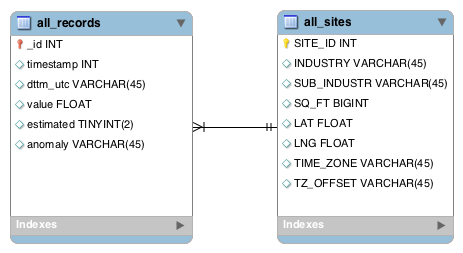
\includegraphics[scale=0.5]{./image/ER.png}
\caption{Entité-Relation relative aux tables de départ fournies pas Enernoc}
\end{figure}

\begin{block}{Note}
Lien entre \sqlcmd{all\_site} et \sqlcmd{all\_records}. Dès les premières injections de données et créations de table il semble évidant que le lien entre ces deux tables nécessite une jointure. Celle-ci se réalise sur les champs : \sqlcmd{all\_sites.SITE\_ID} et \sqlcmd{all\_records}. Comme expliqué en III.1 dans la description des fichiers, les mesures portent en nom de fichier l’id du site mais il ne se retrouve pas dans les colonnes. Nous effectuons donc la jointure sur la méta donnée \sqlcmd{INPUT\_\_FILE\_\_NAME} qui retourne l'adresse complète de la ressource.
(ex: \textcolor{blue}{hdfs://ns3099426....eu:8020/apps/hive/warehouse/project.db/enernoc/474.csv} ) Notre première UDF consistera alors à parser ce chemin pour obtenir l’id, ici \textbf{474}. Cette infomation est accessible pour chaque ligne de la table.
\end{block}

\begin{figure}[h!]
\centering
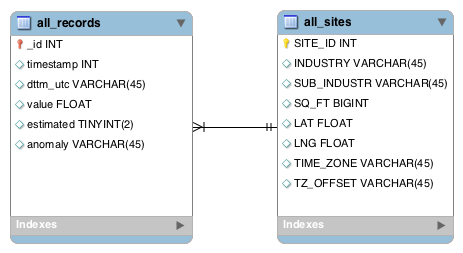
\includegraphics[scale=0.5]{./image/ER.png}
\begin{lstlisting}[language=java]
public Text evaluate(Text input){
  	if (input == null) return new Text("");
		final String path = input.toString();
		final int index = path.lastIndexOf("/");
		final int offset = path.lastIndexOf(".");
		return new Text(path.substring(index + 1, offset));
	}
\end{lstlisting}
\end{figure}

\subsection{Difficultés rencontrées liées à la modélisation: La table colonne}
\subsection{Les solutions privilégiées}


\chapter{Calculs des Load Curves}

\input{./sections/ldone.Rnw}
\input{./sections/ldtwo.Rnw}
\input{./sections/ldthree.Rnw}

\chapter{Data visualisation}

\input{./sections/tableausoftware.Rnw}

\chapter{Conclusion}

\appendix

\chapter{Team work \& code sources du projets}
\section{Workflow de l'équipe Panda}
\section{Exploration et plot sous python}
\section{Recherche des températures avec R}
\chapter{Matériel}
\chapter{Ressources}



\end{document}
